%%%%%%%%%%%%%%%%%%%%%%%%%%%%%%%%%%%%%%%%%
% Lachaise Assignment
% LaTeX Template
% Version 1.0 (26/6/2018)
%
% This template originates from:
% http://www.LaTeXTemplates.com
%
% Authors:
% Marion Lachaise & François Févotte
% Vel (vel@LaTeXTemplates.com)
%
% License:
% CC BY-NC-SA 3.0 (http://creativecommons.org/licenses/by-nc-sa/3.0/)
% 
%%%%%%%%%%%%%%%%%%%%%%%%%%%%%%%%%%%%%%%%

%----------------------------------------------------------------------------------------
%	PACKAGES AND OTHER DOCUMENT CONFIGURATIONS
%----------------------------------------------------------------------------------------

\documentclass{article}

%%%%%%%%%%%%%%%%%%%%%%%%%%%%%%%%%%%%%%%%%
% Lachaise Assignment
% Structure Specification File
% Version 1.0 (26/6/2018)
%
% This template originates from:
% http://www.LaTeXTemplates.com
%
% Authors:
% Marion Lachaise & François Févotte
% Vel (vel@LaTeXTemplates.com)
%
% License:
% CC BY-NC-SA 3.0 (http://creativecommons.org/licenses/by-nc-sa/3.0/)
% 
%%%%%%%%%%%%%%%%%%%%%%%%%%%%%%%%%%%%%%%%%

%----------------------------------------------------------------------------------------
%	PACKAGES AND OTHER DOCUMENT CONFIGURATIONS
%----------------------------------------------------------------------------------------

\usepackage{amsmath,amsfonts,stmaryrd,amssymb,float,graphicx,enumerate,mathtools,listings,xcolor,color,esint,subfig,tikz,pgfplots,setspace,graphicx,array,longtable} % Math packages

\usepackage{enumerate} % Custom item numbers for enumerations

\usepackage[ruled]{algorithm2e} % Algorithms

\usepackage[framemethod=tikz]{mdframed} % Allows defining custom boxed/framed environments

\usepackage{listings} % File listings, with syntax highlighting
\lstset{
	basicstyle=\ttfamily, % Typeset listings in monospace font
}

%----------------------------------------------------------------------------------------
%	DOCUMENT MARGINS
%----------------------------------------------------------------------------------------

\usepackage{geometry} % Required for adjusting page dimensions and margins

\geometry{
	paper=a4paper, % Paper size, change to letterpaper for US letter size
	top=2.5cm, % Top margin
	bottom=3cm, % Bottom margin
	left=2.5cm, % Left margin
	right=2.5cm, % Right margin
	headheight=14pt, % Header height
	footskip=1.5cm, % Space from the bottom margin to the baseline of the footer
	headsep=1.2cm, % Space from the top margin to the baseline of the header
	%showframe, % Uncomment to show how the type block is set on the page
}

%----------------------------------------------------------------------------------------
%	FONTS
%----------------------------------------------------------------------------------------

\usepackage[utf8]{inputenc} % Required for inputting international characters
\usepackage[T1]{fontenc} % Output font encoding for international characters

\usepackage{XCharter} % Use the XCharter fonts

%----------------------------------------------------------------------------------------
%	COMMAND LINE ENVIRONMENT
%----------------------------------------------------------------------------------------

% Usage:
% \begin{commandline}
%	\begin{verbatim}
%		$ ls
%		
%		Applications	Desktop	...
%	\end{verbatim}
% \end{commandline}

\mdfdefinestyle{commandline}{
	leftmargin=10pt,
	rightmargin=10pt,
	innerleftmargin=15pt,
	middlelinecolor=black!50!white,
	middlelinewidth=2pt,
	frametitlerule=false,
	backgroundcolor=black!5!white,
	frametitle={Command Line},
	frametitlefont={\normalfont\sffamily\color{white}\hspace{-1em}},
	frametitlebackgroundcolor=black!50!white,
	nobreak,
}

% Define a custom environment for command-line snapshots
\newenvironment{commandline}{
	\medskip
	\begin{mdframed}[style=commandline]
}{
	\end{mdframed}
	\medskip
}

%----------------------------------------------------------------------------------------
%	FILE CONTENTS ENVIRONMENT
%----------------------------------------------------------------------------------------

% Usage:
% \begin{file}[optional filename, defaults to "File"]
%	File contents, for example, with a listings environment
% \end{file}

\mdfdefinestyle{file}{
	innertopmargin=1.6\baselineskip,
	innerbottommargin=0.8\baselineskip,
	topline=false, bottomline=false,
	leftline=false, rightline=false,
	leftmargin=2cm,
	rightmargin=2cm,
	singleextra={%
		\draw[fill=black!10!white](P)++(0,-1.2em)rectangle(P-|O);
		\node[anchor=north west]
		at(P-|O){\ttfamily\mdfilename};
		%
		\def\l{3em}
		\draw(O-|P)++(-\l,0)--++(\l,\l)--(P)--(P-|O)--(O)--cycle;
		\draw(O-|P)++(-\l,0)--++(0,\l)--++(\l,0);
	},
	nobreak,
}

% Define a custom environment for file contents
\newenvironment{file}[1][File]{ % Set the default filename to "File"
	\medskip
	\newcommand{\mdfilename}{#1}
	\begin{mdframed}[style=file]
}{
	\end{mdframed}
	\medskip
}

%----------------------------------------------------------------------------------------
%	NUMBERED QUESTIONS ENVIRONMENT
%----------------------------------------------------------------------------------------

% Usage:
% \begin{question}[optional title]
%	Question contents
% \end{question}

\mdfdefinestyle{question}{
	innertopmargin=1.2\baselineskip,
	innerbottommargin=0.8\baselineskip,
	roundcorner=5pt,
	nobreak,
	singleextra={%
		\draw(P-|O)node[xshift=1em,anchor=west,fill=white,draw,rounded corners=5pt]{%
		Question \theQuestion\questionTitle};
	},
}

\newcounter{Question} % Stores the current question number that gets iterated with each new question

% Define a custom environment for numbered questions
\newenvironment{question}[1][\unskip]{
	\bigskip
	\stepcounter{Question}
	\newcommand{\questionTitle}{~#1}
	\begin{mdframed}[style=question]
}{
	\end{mdframed}
	\medskip
}

%----------------------------------------------------------------------------------------
%	WARNING TEXT ENVIRONMENT
%----------------------------------------------------------------------------------------

% Usage:
% \begin{warn}[optional title, defaults to "Warning:"]
%	Contents
% \end{warn}

\mdfdefinestyle{warning}{
	topline=false, bottomline=false,
	leftline=false, rightline=false,
	nobreak,
	singleextra={%
		\draw(P-|O)++(-0.5em,0)node(tmp1){};
		\draw(P-|O)++(0.5em,0)node(tmp2){};
		\fill[black,rotate around={45:(P-|O)}](tmp1)rectangle(tmp2);
		\node at(P-|O){\color{white}\scriptsize\bf !};
		\draw[very thick](P-|O)++(0,-1em)--(O);%--(O-|P);
	}
}

% Define a custom environment for warning text
\newenvironment{warn}[1][Warning:]{ % Set the default warning to "Warning:"
	\medskip
	\begin{mdframed}[style=warning]
		\noindent{\textbf{#1}}
}{
	\end{mdframed}
}

%----------------------------------------------------------------------------------------
%	INFORMATION ENVIRONMENT
%----------------------------------------------------------------------------------------

% Usage:
% \begin{info}[optional title, defaults to "Info:"]
% 	contents
% 	\end{info}

\mdfdefinestyle{info}{%
	topline=false, bottomline=false,
	leftline=false, rightline=false,
	nobreak,
	singleextra={%
		\fill[black](P-|O)circle[radius=0.4em];
		\node at(P-|O){\color{white}\scriptsize\bf i};
		\draw[very thick](P-|O)++(0,-0.8em)--(O);%--(O-|P);
	}
}

% Define a custom environment for information
\newenvironment{info}[1][Info:]{ % Set the default title to "Info:"
	\medskip
	\begin{mdframed}[style=info]
		\noindent{\textbf{#1}}
}{
	\end{mdframed}
}

\pgfplotsset{compat=1.12}
\usepgfplotslibrary{fillbetween}
\DeclareMathOperator{\sech}{sech}
\DeclareMathOperator{\arcsech}{arcsech}
\DeclareMathOperator{\arcoth}{arcoth}
\DeclareMathOperator{\arctanh}{tanh^{-1}}
\renewcommand{\baselinestretch}{1.25}
\newcommand{\bin}{\sf Bin}
\newcommand{\G}{\sf G}
\newcommand{\Hyp}{\sf Hyp}
\newcommand{\Po}{\sf Po}
\newcommand{\ex}{\sf Exp}
\newcommand{\Nor}{\sf N}
\newcommand{\gam}{\sf Gam} 
\newcommand{\Em}{\mathbb E}
\newcommand{\Pm}{\mathbb P}
\newcommand{\R}{\mathbb R}
\newcommand{\B}{\cal B}
\newcommand{\N}{\mathbb N}
\newcommand{\Z}{\mathbb Z}
\newcommand{\Q}{\mathbb Q}
\newcommand{\Comp}{\mathbb C}
\newcommand{\e}{\mbox{e}}
\newcommand{\Var}{\mbox{Var}}
\newcommand{\cov}{\mbox{Cov}}
\newcommand{\ds}{\displaystyle}
\newcommand{\subvect}[1]{\mbox{\small \boldmath #1}}
%\newcommand{\vect}[1]{\mbox{\boldmath $#1$}}
\newcommand{\vect}[1]{\boldsymbol #1}
\newcommand{\norm}[1]{\left\lVert#1\right\rVert}
\newcommand*\VF[1]{\mathbf{#1}}
\newcommand*\dif{\mathop{}\!\mathrm{d}}
\setlength{\jot}{7pt}
\definecolor{lbcolor}{rgb}{0.95,0.95,0.95}
\usepackage{amsmath,amssymb}

\title{COMS3200: Revision} % Title of the document
\author{Team Collusion}
\date{University of Queensland --- \today}
\begin{document}

\maketitle % Print the title

\section*{Ch 1. Introduction}
\noindent
\rule{\linewidth}{0.5mm}
\noindent

\subsection*{Misc definitions, Sections 1.1 - 1.2.1}
\begin{description}
    \item[Internet] The Internet is the global system of interconnected computer networks that use the Internet protocol suite (TCP/IP) to link devices worldwide. It is a network of networks that consists of private, public, academic, business, and government networks of local to global scope, linked by a broad array of electronic, wireless, and optical networking technologies. The Internet carries a vast range of information resources and services, such as the inter-linked hypertext documents and applications of the World Wide Web (WWW), electronic mail, telephony, and file sharing.
    
    \item[Network Hosts/End systems] A network host is a computer connected to a computer network. A host may work as a server offering information resources, services, and applications to users or other nodes on the network. Hosts are assigned at least one network address.
    
    \item[Internet Protocol (IP)] The Internet Protocol (IP) is the principal communications protocol in the Internet protocol suite for relaying datagrams across network boundaries. Its routing function enables internetworking, and essentially establishes the Internet. IP has the task of delivering packets from the source host to the destination host solely based on the IP addresses in the packet headers. For this purpose, IP defines packet structures that encapsulate the data to be delivered. It also defines addressing methods that are used to label the datagram with source and destination information. Historically, IP was the connectionless datagram service in the original Transmission Control Program introduced by Vint Cerf and Bob Kahn in 1974, which was complemented by a connection-oriented service that became the basis for the Transmission Control Protocol (TCP). The Internet protocol suite is therefore often referred to as TCP/IP. The first major version of IP, Internet Protocol Version 4 (IPv4), is the dominant protocol of the Internet. Its successor, Internet Protocol Version 6 (IPv6), has been growing in adoption, 

    \item[Distributed Computing] Distributed computing is a field of computer science that studies distributed systems. A distributed system is a system whose components are located on different networked computers, which communicate and coordinate their actions by passing messages to one another. The components interact with one another in order to achieve a common goal. Three significant characteristics of distributed systems are: concurrency of components, lack of a global clock, and independent failure of components. Examples of distributed systems vary from SOA-based systems to massively multiplayer online games to peer-to-peer applications.
     
    \item[Network Protocols] A network protocol defines the format and the order of messages exchanged between
    two or more communicating entities, as well as the actions taken on the transmission
    and/or receipt of a message or other event.

    \item[Clients] A client is a computer or a program that, as part of its operation, relies on sending a request to another program or a computer hardware or software that accesses a service made available by a server(which may or may not be located on another computer). For example, web browsers are clients that connect to web servers and retrieve web pages for display. Email clients retrieve email from mail servers. Online chat uses a variety of clients, which vary depending on the chat protocol being used. Multiplayer video games or online video games may run as a client on each computer. The term "client" may also be applied to computers or devices that run the client software or users that use the client software.
    
    \item[Servers] In computing, a server is a computer program or a device that provides functionality for other programs or devices, called "clients". This architecture is called the client–server model, and a single overall computation is distributed across multiple processes or devices. Servers can provide various functionalities, often called "services", such as sharing data or resources among multiple clients, or performing computation for a client. A single server can serve multiple clients, and a single client can use multiple servers. A client process may run on the same device or may connect over a network to a server on a different device. Typical servers are database servers, file servers, mail servers, print servers, web servers, game servers, and application servers.
    
    \item[Client-Server model] Client–server model is a distributed application structure that partitions tasks or workloads between the providers of a resource or service, called servers, and service requesters, called clients. Often clients and servers communicate over a computer network on separate hardware, but both client and server may reside in the same system. A server host runs one or more server programs which share their resources with clients. A client does not share any of its resources, but requests a server's content or service function. Clients therefore initiate communication sessions with servers which await incoming requests. Examples of computer applications that use the client–server model are Email, network printing, and the World Wide Web.
    
    \item[Digital Subscriber Line (DSL)] Digital subscriber line (DSL; originally digital subscriber loop) is a family of technologies that are used to transmit digital data over telephone lines. In telecommunications marketing, the term DSL is widely understood to mean asymmetric digital subscriber line (ADSL), the most commonly installed DSL technology, for Internet access. DSL service can be delivered simultaneously with wired telephone service on the same telephone line since DSL uses higher frequency bands for data. On the customer premises, a DSL filter on each non-DSL outlet blocks any high-frequency interference to enable simultaneous use of the voice and DSL services. A residence typically obtains DSL Internet access
    from the same local telephone company (telco) that provides its wired local phone
    access. Thus, when DSL is used, a customer’s telco is also its ISP. Eeach customer’s DSL modem uses the existing telephone line to exchange data with a digital
    subscriber line access multiplexer (DSLAM) located in the telco’s local central
    office (CO). The home’s DSL modem takes digital data and translates it to highfrequency
    tones for transmission over telephone wires to the CO; the analog signals
    from many such houses are translated back into digital format at the DSLAM.
    The residential telephone line carries both data and traditional telephone signals
    simultaneously, which are encoded at different frequencies:
    \begin{itemize}
        \item A high-speed downstream channel, in the 50 kHz to 1 MHz band
        \item A medium-speed upstream channel, in the 4 kHz to 50 kHz band
        \item An ordinary two-way telephone channel, in the 0 to 4 kHz band
    \end{itemize}
    This approach makes the single DSL link appear as if there were three separate
    links, so that a telephone call and an Internet connection can share the DSL link at
    the same time. On the customer side, a splitter separates the data and telephone signals
    arriving to the home and forwards the data signal to the DSL modem. On the
    telco side, in the CO, the DSLAM separates the data and phone signals and sends
    the data into the Internet. Hundreds or even thousands of households connect to a
    single DSLAM [Dischinger 2007]. The DSL standards define transmission rates of 12 Mbps downstream and
    1.8 Mbps upstream [ITU 1999], and 24 Mbps downstream and 2.5 Mbps upstream
    [ITU 2003]. Because the downstream and upstream rates are different, the access is
    said to be asymmetric. The actual downstream and upstream transmission rates
    achieved may be less than the rates noted above, as the DSL provider may purposefully
    limit a residential rate when tiered service (different rates, available at different
    prices) are offered, or because the maximum rate can be limited by the distance
    between the home and the CO, the gauge of the twisted-pair line and the degree of
    electrical interference. Engineers have expressly designed DSL for short distances
    between the home and the CO; generally, if the residence is not located within 5 to 10
    miles of the CO, the residence must resort to an alternative form of Internet access.

    \item[Cable Internet access] In telecommunications, cable Internet access, shortened to cable Internet, is a form of broadband Internet access which uses the same infrastructure as a cable television. Like digital subscriber line and fiber to the premises services, cable Internet access provides network edge connectivity (last mile access) from the Internet service provider to an end user. It is integrated into the cable television infrastructure analogously to DSL which uses the existing telephone network. Cable TV networks and telecommunications networks are the two predominant forms of residential Internet access. Cable Internet access makes use of the cable television company’s existing cable
    television infrastructure. A residence obtains cable Internet access from the same
    company that provides its cable television. Fiber optics
    connect the cable head end to neighborhood-level junctions, from which traditional
    coaxial cable is then used to reach individual houses and apartments. Each
    neighborhood junction typically supports 500 to 5,000 homes. Because both fiber
    and coaxial cable are employed in this system, it is often referred to as hybrid
    fiber coax (HFC). One important characteristic of cable Internet access is that it is a shared
    broadcast medium. In particular, every packet sent by the head end travels downstream
    on every link to every home and every packet sent by a home travels on the
    upstream channel to the head end. For this reason, if several users are simultaneously
    downloading a video file on the downstream channel, the actual rate at which
    each user receives its video file will be significantly lower than the aggregate cable
    downstream rate. On the other hand, if there are only a few active users and they
    are all Web surfing, then each of the users may actually receive Web pages at the
    full cable downstream rate, because the users will rarely request a Web page at
    exactly the same time. Because the upstream channel is also shared, a distributed
    multiple access protocol is needed to coordinate transmissions and avoid collisions.
\end{description}

\subsection*{Physical Media (Section 1.2.2)}

\begin{description}
    \item[Twisted-Pair Copper Wire] The least expensive and most commonly used guided transmission medium is
    twisted-pair copper wire. For over a hundred years it has been used by telephone
    networks. In fact, more than 99 percent of the wired connections from the telephone
    handset to the local telephone switch use twisted-pair copper wire. Most of
    us have seen twisted pair in our homes and work environments. Twisted pair consists
    of two insulated copper wires, each about 1 mm thick, arranged in a regular
    spiral pattern. The wires are twisted together to reduce the electrical interference
    from similar pairs close by. Typically, a number of pairs are bundled together in a
    cable by wrapping the pairs in a protective shield. A wire pair constitutes a single
    communication link. {\bf Unshielded twisted pair (UTP)} is commonly used for computer networks within a building, that is, for LANs. Data rates for LANs
    using twisted pair today range from 10 Mbps to 10 Gbps. The data rates that can
    be achieved depend on the thickness of the wire and the distance between transmitter
    and receiver.

    \item[Coaxial Cable] Like twisted pair, coaxial cable consists of two copper conductors, but the two conductors are concentric rather than parallel. With this construction and special insulation
    and shielding, coaxial cable can achieve high data transmission rates. Coaxial
    cable is quite common in cable television systems. As we saw earlier, cable television
    systems have recently been coupled with cable modems to provide residential
    users with Internet access at rates of tens of Mbps. In cable television and cable
    Internet access, the transmitter shifts the digital signal to a specific frequency band,
    and the resulting analog signal is sent from the transmitter to one or more receivers.
    Coaxial cable can be used as a guided shared medium. Specifically, a number of
    end systems can be connected directly to the cable, with each of the end systems
    receiving whatever is sent by the other end systems.

    \item[Fiber Optics] An optical fiber is a thin, flexible medium that conducts pulses of light, with each
    pulse representing a bit. A single optical fiber can support tremendous bit rates, up
    to tens or even hundreds of gigabits per second. They are immune to electromagnetic
    interference, have very low signal attenuation up to 100 kilometers, and are
    very hard to tap. These characteristics have made fiber optics the preferred longhaul
    guided transmission media, particularly for overseas links. Many of the longdistance
    telephone networks in the United States and elsewhere now use fiber optics
    exclusively. Fiber optics is also prevalent in the backbone of the Internet. However,
    the high cost of optical devices—such as transmitters, receivers, and switches—has
    hindered their deployment for short-haul transport, such as in a LAN or into the
    home in a residential access network. The Optical Carrier (OC) standard link speeds
    range from 51.8 Mbps to 39.8 Gbps; these specifications are often referred to as OCn,
    where the link speed equals n × 51.8 Mbps.

    \item[Terrestrial Radio Channels] Radio channels carry signals in the electromagnetic spectrum. They are an attractive
    medium because they require no physical wire to be installed, can penetrate walls,
    provide connectivity to a mobile user, and can potentially carry a signal for long distances.
    The characteristics of a radio channel depend significantly on the propagation
    environment and the distance over which a signal is to be carried. Environmental considerations
    determine path loss and shadow fading (which decrease the signal strength
    as the signal travels over a distance and around/through obstructing objects), multipath
    fading (due to signal reflection off of interfering objects), and interference (due
    to other transmissions and electromagnetic signals).
    Terrestrial radio channels can be broadly classified into three groups: those that
    operate over very short distance (e.g., with one or two meters); those that operate in
    local areas, typically spanning from ten to a few hundred meters; and those that
    operate in the wide area, spanning tens of kilometers. Personal devices such as wireless
    headsets, keyboards, and medical devices operate over short distances; the
    wireless LAN technologies use local-area radio channels;
    the cellular access technologies use wide-area radio channels.

    \item[Satellite Radio Channels] A communication satellite links two or more Earth-based microwave transmitter/
    receivers, known as ground stations. The satellite receives transmissions on one frequency
    band, regenerates the signal using a repeater (discussed below), and transmits
    the signal on another frequency. Two types of satellites are used in communications:
    geostationary satellites and low-earth orbiting (LEO) satellites.
    Geostationary satellites permanently remain above the same spot on Earth. This
    stationary presence is achieved by placing the satellite in orbit at 36,000 kilometers
    above Earth’s surface. This huge distance from ground station through satellite back
    to ground station introduces a substantial signal propagation delay of 280 milliseconds.
    Nevertheless, satellite links, which can operate at speeds of hundreds of Mbps,
    are often used in areas without access to DSL or cable-based Internet access.
    LEO satellites are placed much closer to Earth and do not remain permanently
    above one spot on Earth. They rotate around Earth (just as the Moon does) and may
    communicate with each other, as well as with ground stations.
\end{description}


\subsection*{Network Core (Section 1.3)}

\begin{description}
    \item[Packet-Switching] 
    Uses \textit{store and forward} idea: entire packet must arrive at router before it can be
    transmitted on the next link. Takes $\frac LR$ seconds to transmit entire $L$-bit packet into 
    link at $R$bps. Thus, end-to-end delay is $2\frac LR$, assuming same bps at both ends.
    If the arrival rate in bits exceeds transmission rate of link, packets are queued in a buffer.
    Packet loss occurs when packet arrives and buffer is full. Protocols must supply congestion
    control and reliable data transfer.
    
    \item[Circuit Switching]
    End-to-end resources allocated and reserved for duration of communication between source and 
    destination. Resources are dedicated, so circuit-like performance is guaranteed, however segment
    is idle if not being used and thus wasted resources. Can allocate resources using Frequency
    Division Multiplexing (certain frequency allocated per user) or Time Division Multiplexing
    (certain time frame allocated per user).
\end{description}

\subsection*{Delay and Throughput (Section 1.4)}

Total delay at a node (router) is given by
\[
    d_{\text{nodal}} = d_{\text{proc}} + d_{\text{queue}} + d_{\text{trans}} + d_{\text{prop}}.
\]
% NOTE: Maybe include A1 PART A as an example?
\begin{description}
    \item[Processing delay]
    Time used to check bits for errors and determine output link for packet.
    
    \item[Queueing delay]
    Time spend in the queue waiting out output link for transmission, depending largely on level of
    congestion at router.
    
    \item[Transmission delay]
    Determined by $\frac LR$ where $L$ is the length of the packet in bits and $R$ is the link 
    bandwidth in bps.
    
    \item[Propagation delay]
    Given by $\frac ds$ where $d$ is the length (distance) of the physical link and $s$ is the 
    propagation speed.
    
    \item[Throughput]
    The rate at which bits are transferred between sender/receiver, measured in bits per time unit 
    (different from delay). If a server has a throughput of $R_s$bps and a client has a throughput of
    $R_c$bps, then a bottleneck occurs at $\min\{R_c,R_s\}.$
\end{description}


\subsection*{Protocol Layers and Their Service Models (Section 1.5)}

\begin{description}
    \item[Layers] To provide structure to the design of network protocols, network designers organize protocols and the network hardware and software that implement the protocols in layers. A layer serves the layer above it and is served by the layer below it. For example, a layer that provides error-free communications across a network provides the path needed by applications above it, while it calls the next lower layer to send and receive packets that constitute the contents of that path. Each protocol belongs to one of the layers. Layering provides a way of hiding the working details of a subsystem, allowing the separation of concerns to facilitate interoperability and platform independence.
    
    \begin{figure}[H]
        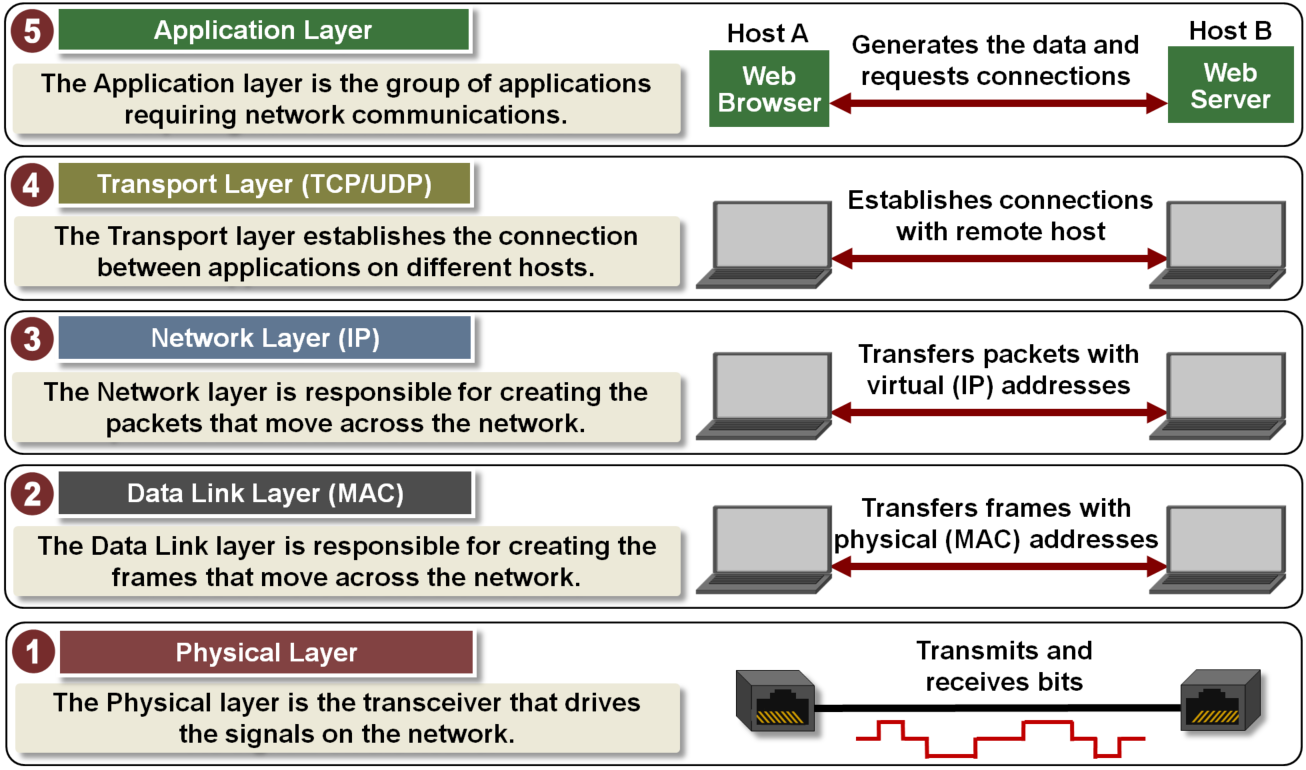
\includegraphics[scale=0.5]{images/5_layer_overview.png}
        \centering
        \caption{Pictorial Layer Summary (bc we all love pictures!)}
    \end{figure}
    
    \begin{description}
        \item[Application Layer] The application layer is where network applications and their application layer protocols reside. The Internet’s application layer includes many protocols, such as the HTTP protocol (which provides for Web document request and transfer), SMTP (which provides for the transfer of e-mail messages), and FTP (which provides for the transfer of files between two end systems). An application-layer protocol is distributed over multiple end systems, with the
        application in one end system using the protocol to exchange packets of information
        with the application in another end system. We’ll refer to this packet of information
        at the application layer as a {\bf message}.
        
        \item[Transport Layer] The Internet’s transport layer transports application-layer messages between
        application endpoints. In the Internet there are two transport protocols, TCP and
        UDP, either of which can transport application-layer messages. TCP provides a
        connection-oriented service to its applications. This service includes guaranteed
        delivery of application-layer messages to the destination and flow control (that is,
        sender/receiver speed matching). TCP also breaks long messages into shorter segments
        and provides a congestion-control mechanism, so that a source throttles its
        transmission rate when the network is congested. The UDP protocol provides a connectionless
        service to its applications. This is a no-frills service that provides no
        reliability, no flow control, and no congestion control. In this book, we’ll refer to a
        transport-layer packet as a {\bf segment}.
        
        \item[Network Layer] The Internet’s network layer is responsible for moving network-layer packets
        known as {\bf datagrams} from one host to another. The Internet transport-layer protocol
        (TCP or UDP) in a source host passes a transport-layer segment and a destination
        address to the network layer, just as you would give the postal service a letter
        with a destination address. The network layer then provides the service of delivering
        the segment to the transport layer in the destination host.
        The Internet’s network layer includes the celebrated IP Protocol, which defines
        the fields in the datagram as well as how the end systems and routers act on these
        fields. There is only one IP protocol, and all Internet components that have a network
        layer must run the IP protocol. The Internet’s network layer also contains routing
        protocols that determine the routes that datagrams take between sources and destinations. The Internet has many routing protocols.
        
        \item[Link Layer] The Internet’s network layer routes a datagram through a series of routers between
        the source and destination. To move a packet from one node (host or router) to the
        next node in the route, the network layer relies on the services of the link layer. In
        particular, at each node, the network layer passes the datagram down to the link
        layer, which delivers the datagram to the next node along the route. At this next
        node, the link layer passes the datagram up to the network layer.
        The services provided by the link layer depend on the specific link-layer protocol
        that is employed over the link. For example, some link-layer protocols provide
        reliable delivery, from transmitting node, over one link, to receiving node. Note that
        this reliable delivery service is different from the reliable delivery service of TCP,
        which provides reliable delivery from one end system to another. Examples of linklayer
        protocols include Ethernet, WiFi, and the cable access network’s DOCSIS protocol.
        As datagrams typically need to traverse several links to travel from source to
        destination, a datagram may be handled by different link-layer protocols at different
        links along its route. For example, a datagram may be handled by Ethernet on one
        link and by PPP on the next link. The network layer will receive a different service
        from each of the different link-layer protocols. In this book, we’ll refer to the linklayer
        packets as {\bf frames}.
        
        \item[Physical Layer] While the job of the link layer is to move entire frames from one network element
        to an adjacent network element, the job of the physical layer is to move the individual
        bits within the frame from one node to the next. The protocols in this layer are
        again link dependent and further depend on the actual transmission medium of the
        link (for example, twisted-pair copper wire, single-mode fiber optics). For example,
        Ethernet has many physical-layer protocols: one for twisted-pair copper wire,
        another for coaxial cable, another for fiber, and so on. In each case, a bit is moved
        across the link in a different way.
    \end{description}
    
    \item[Examples of each layer]$\hfill$
    \begin{enumerate}
            \item[5.] \textbf{Application Layer}: supporting network application (FTP, SMTP, HTTP)
            \item[4.] \textbf{Transport Layer}: process-process data transfer (TCP, UDP)
            \item[3.] \textbf{Network Layer}: routing of datagrams from source to destination (IP, routing 
            protocols)
            \item[2.] \textbf{Link Layer}: data transfer between neighbouring network elements (Ethernet, 
            Wifi, ARP)
            \item[1.] \textbf{Physical Layer}: bits ``on the wire'' (or spectrum)
    \end{enumerate}
    
    
\end{description}

\section*{Ch 2. Application Layer}
\noindent
\rule{\linewidth}{0.5mm}
\noindent

\subsection*{Principles of network applications (Section ?.?.?)}

\begin{description}
    \item[Client-Server model] An ``always-on'' \textbf{server} acts as a host, with a permanent IP 
    address, so that a \textbf{client} may intermittently connect with the server. Clients may have
    dynamic IP addresses and communicate only with the server, never between other clients. 
    Processes running in this model are either a client process (one which initiates communication)
    or a server process (one which waits to be contacted).
    
    \item[P2P Architecture] There is no ``always-on server''; peers request service from other peers
    and also provide a service if another peer requests it. They are intermittently connected and
    may change IP addresses. Peers communicate directly with each other. Processes act as a client
    and server process.
\end{description}

\subsection*{Web and HTTP (Section ?.?.?)}

\begin{description}
    \item[Round Trip Time (RTT)] Time for a small packet to travel from the client to the server and
    back.
    
    \item[Non-persistent HTTP] At most one object is sent over a TCP connection, which is then closed
    after it is received. Therefore, downloading multiple objects required multiple connections with 
    the server. When requesting an object, the total time taken $2RTT+\text{file transmission time}$.
    This occurs per object, so when requesting multiple objects, browsers often open parallel TCP
    connections to fetch each.
    
    \item[Persistent HTTP] Multiple objects can be sent over a single TCP connection, as the server
    leaves the connection open after sending its response. A client sends a request as soon as it 
    encounters a referenced object, so as little as $1RTT$ is required for all objects, since the 
    same open connection is used.
    
    \item[HTTP Request]
    A HTTP request message is formatted as
    \begin{align*}
        &\texttt{METHOD REQUEST-URI HTTP-VERSION\textbackslash r\textbackslash n}\\
        &\texttt{REQUEST-HEADER\textbackslash r\textbackslash n}\\
        &\dots\\
        &\texttt{\textbackslash r\textbackslash n}
    \end{align*}
    where $\texttt{METHOD}\in\{\texttt{GET, POST, HEAD}\}$ and
    \begin{align*}
        \texttt{REQUEST-HEADER}\in\{&\texttt{Accept, \dots, Authorization, Expect, From, Host, If-Match,}\\
        &\texttt{If-Modified-Since,\dots, If-Unmodified-since, User-Agent,\dots}\}.
    \end{align*}
    
        \item[HTTP Response]
    A HTTP response message is formatted as
    \begin{align*}
        &\texttt{HTTP-VERSION STATUS-CODE REASON-PHRASE\textbackslash r\textbackslash n}\\
        &\texttt{RESPONSE-HEADER\textbackslash r\textbackslash n}\\
        &\dots\\
        &\texttt{\textbackslash r\textbackslash n}\\
        &\texttt{[message body]}
    \end{align*}
    where \texttt{STATUS-CODE} and \texttt{REASON-PHRASE} are given by
    \begin{enumerate}
        \item[100] Continue
        \item[200] OK
        \item[301] Moved Permanently
        \item[400] Bad Request
        \item[401] Unauthorized
        \item[403] Forbidden
        \item[404] Not Found
        \item[500] Internal Server Error
        \item[502] Bad Gateway
    
        \item[1xx] Informational - Request received, continuing process
        \item[2xx] Success - The action was successfully received, understood, and accepted
        \item[3xx] Redirection - Further action must be taken in order to complete the request
        \item[4xx] Client Error - The request contains bad syntax or cannot be fulfilled
        \item[5xx] Server Error - The server failed to fulfill an apparently valid request
    \end{enumerate}
    among others and 
    \[
        \texttt{RESPONSE-HEADER}\in\{\texttt{Accept-Ranges, Last-Modified, Content-Length, Content-type\dots}\}.
    \]
    
    \item[Cookies] May be used to keep information about the ``state'' between the client and the 
    server. Can be used for authorization, shopping carts, recommendations, etc.
    
    \item[Web Caches] A proxy server may be used to cache common HTTP requests for faster response 
    times. If an object is in the cache, then the proxy server returns it to the requesting client.
    If it is not in the cache, the proxy forwards the request to the server, then forwards the 
    servers response to the client and caches it.
\end{description}

\subsection*{E-mail (Section ?.?)}

\begin{description}
    \item[User Agent] The ``mail reader'' and is used to compose, edit, read, etc mail messages.
    Outgoing and incoming messages are stored on the server. Examples include Outlook, Thunderbird, etc.
    
    \item[Mail server] Contains \textbf{mailbox} of incoming messages for a user and a \textbf{message queue}
    of outgoing (to be sent) mail messages.
    
    \item[Simple Mail Transfer Protocol(SMTP)] for sending messages between mail servers. Uses TCP on
    port 25 as a persistent connection. Contains a handshake, transfer of messages and closure in a
    command/response like interaction.
    
    \item[Mail Access protocols] For retrieving mail from a mail server. Eg POP, IMAP, HTTP.
\end{description}

\subsection*{DNS: Domain Name System (Section ?.?.?)}

\begin{description}
    \item[Services/Structure] Hostname (e.g google.com) to IP address translation. It is implemented
    in a hierarchy of many \textbf{name servers}, which communicate to resolve names (translate).
    There are $13$ logical root name servers world wide, though they are replicated many times.
    
    \item[Top-level domain server (TLD)] Responsible for com, org, net, edu, aero, jobs, museums and 
    all top-level country domains.
    
    \item[Authoritative DNS serves] Organizations own DNS server, providing hostname to IP mappings
    for organizations named hosts.
    
    \item[Local DNS name server] Each ISP may maintain their own. When a DNS request is sent from a 
    host, it is sent to this server. It has a cache of recent requests and acts as a proxy, forwarding
    requests into the hierarchy.
    
    \item[Iterated Query] When the contacted server replies with the name of some other server to 
    contact in order to resolve the request.
    
    \item[Recursive Query] When the contacted server determines the name resolution on its own. It 
    may contact other servers which in turn do this, hence ``recursive.''
    
    \item[Record types] DNS is essentially a distributed database storing resource records (RR) of 
    the form \\
    $(\texttt{name, value, type, ttl})$ where $\texttt{type}\in\{\texttt{A, NS, CNAME, 
    MX}\}$:
    \begin{description}
        \item[A] \texttt{name} is hostname and \texttt{value} is IP address.
        \item[NS] \texttt{name} is domain (foo.com) and \texttt{value} is hostname of authoritative
        name server for this domain
        \item[CNAME] \texttt{name} is alias for some canonical (real) name and \texttt{value} is 
        canocnical name
        \item[MX] \texttt{value} is name of mailserver associated with \texttt{name}.
    \end{description}
    
    \item[DNS format] A DNS message looks like
    %TODO insert image
    
    \item[Attacking DNS] Root and TLD servers may be inundated with traffic in order a denial of 
    service attack. Can also intercept queries from DNS servers and send bogus replies to them, which
    are usually cached.
\end{description}

\section*{Ch 3. Transport Layer}
\noindent
\rule{\linewidth}{0.5mm}
\noindent

\subsection*{Principles of Transport Layer protocols}

\begin{description}
    \item[Services] Provides logical communication between app processes running on different hosts.
    Sender breaks app message into segments, which are passed to the network layer whereas receiver
    reassembles segments into app message and passes them up to application layer.
    
    \item[Multiplexing] Done at sender-side and handles data from multiple sockets, adding the 
    transport layer header.
    
    \item[Demultiplexing] Done at receiver-side and uses header info to deliver received segments to
    the correct socket. In a connectionless protocol, only the destination port number and IP 
    address is used to determine which socket to send the received data through. In a
    connection-orientated protocol, the source and destination addresses and port numbers are used to
    uniquely identify a socket.
\end{description}

\subsection*{User Datagram Protocol (UDP)}

\begin{description}
    \item[Connectionless] No handshake between sender and receiver; each UDP segment is handled
    independently of others. Segments may be lost or delivered out-of-order, in which case it is up
    to the application to handle this re-request or reorder the segments. Used as there is no handshake
    (meaning no delay), it is simple, small header size and there is no congestion control so segments
    can be sent as fast as desired.
    
    \item[Checksum] Used to detect errors in transmitted segment. A sender computes the checksum by
    treating all data in the datagram (header + payload) as 16bit words and adds them together using
    one's complement sum and puts the result in the ``checksum'' header field. A receiver then adds
    all 16bit values of header and payload: if the result is $0$, no error is detected, else an error
    is detected.
    
    \item[Header] A typical UDP header looks like 
    %TODO include figure
\end{description}

\subsection*{Reliable Data Transfer}

\begin{description}
    \item[RDT1.0] Base step for building RDT. Sender will
    \begin{enumerate}
        \item Wait for call from above
        \item Make the segment and send it
        \item Repeat above process
    \end{enumerate}
    Receiver will
    \begin{enumerate}
        \item Wait for call from below
        \item Extract data from segment and push it to above layer
        \item Repeat above process
    \end{enumerate}
    
    \item[RDT2.0] Adds error detection via checksum and feedback via ACK/NAK. Sender will
    \begin{enumerate}
        \item Wait for call from above
        \item Make segment and send it
        \item Wait for response. If response is NAK repeat step, else (ACK received) continue
        \item Repeat above process
    \end{enumerate}
    Receiver will
    \begin{enumerate}
        \item Wait for call from below
        \item If received packet is corrupted send NAK, else extract data and push it to above layer 
        and send ACK
        \item Repeat above process
    \end{enumerate}
    
    \item[RDT2.1] Adds sequence numbers to segments. Sender will
    \begin{enumerate}
        \item Wait for call from above with seq=0
        \item Make segment with seq=0 and send it
        \item Wait for response with ACK or NAK and seq=0. If response is NAK or corrupted repeat last step,
        else continue
        \item Wait for call form above with seq=1
        \item Make segment with seq=1 and send it
        \item Wait for response with ACK or NAK and seq=1. If response is NAK or corrupted repeat last step,
        else continue
        \item Repeat above process
    \end{enumerate}
    Receiver will
    \begin{enumerate}
        \item Wait for call form below with seq=0
        \item If response with has seq=1 send ACK and repeat last step. If response is corrupted send 
        NAK and repeat last step. If response is not corrupted and has seq=0 extract data and push it 
        to above layer and send ACK
        \item Wait for call from below with seq=1
        \item If response with has seq=0 send ACK and repeat last step. If response is corrupted send 
        NAK and repeat last step. If response is not corrupted and has seq=1 extract data and push it 
        to above layer and send ACK
        \item Repeat above process
    \end{enumerate}
    
    \item[RDT2.2] Removes NAK by only sending ACK for last received segment if OK. Sender will
    \begin{enumerate}
        \item Wait for call from above with seq=0
        \item Make segment with seq=0 and send it
        \item Wait for response with ACK and seq=0. If response is corrupted repeat last step,
        else continue
        \item Wait for call form above with seq=1
        \item Make segment with seq=1 and send it
        \item Wait for response with ACK and seq=1. If response is corrupted repeat last step,
        else continue
        \item Repeat above process
    \end{enumerate}
    Receiver will
    \begin{enumerate}
        \item Wait for call form below with seq=0
        \item If response with has seq=1 resend packet and repeat last step. If response is not
        corrupted and has seq=0 extract data and push it to above layer and send ACK
        \item Wait for call from below with seq=1
        \item If response with has seq=0 send ACK and repeat last step. If response is corrupted send 
        NAK and repeat last step. If response is not corrupted and has seq=1 extract data and push it 
        to above layer and send ACK with seq=1
        \item Repeat above process
    \end{enumerate}
    
    \item[RDT3.0] Sender now waits a ``reasonable'' amount of time for ACK. Sender will
    \begin{enumerate}
        \item Wait for call from above with seq=0
        \item Make segment with seq=0, send it and start timer
        \item Wait for response with ACK and seq=0. If response is corrupted do nothing. If timeout occurs, repeat last step else stop timer and continue
        \item Wait for call form above with seq=1
        \item Make segment with seq=1, send it and start timer
        \item Wait for response with ACK and seq=1. If response is corrupted do nothing. If timeout
        occurs, repeat last step else stop timer and continue
        \item Repeat above process 
    \end{enumerate}
    Receiver does not change from RDT2.2.
    
    \item[Pipelining] Window size of $N$ is used to transmit $N$ segments at a time. Only when the
    smallest segment is acked can the window be advanced.
    
    \item[Go-back-N] Sender can have up to $N$ unacked segments in the pipeline and only has timer for
    the last unacked segment. On timeout, the previous $N$ segments are retransmitted. The receiver
    only sends an ACK for the highest received \textit{in-order} segment. If a segment is received
    out of order, it is discarded. An ACK acks all previous segments.
    
    \item[Selective repeat] Receiver \textit{individually} acks all correctly received segments and
    buffers segments as needed for eventual in-order delivery to upper layer. The sender only re-sends
    segments for which it did not receive an ACK.
\end{description}

\subsection*{Transmission Control Protocol (TCP)}

\begin{description}
    \item[Connection-oriented] There is one sender and one receiver per socket. A three-way handshake
    is used to initiate communication between sender and receiver. Provides reliable in-order byte stream,
    flow control and connection management. The sequence number in a TCP header is the byte stream
    number of the first byte in the segments data. The acknowledgement number is the sequence number
    of the next expected byte. 
    
    \item[RTT/Timeouts] RTT is estimated by measuring time from segment transmit until ACK receipt.
    Average RTT is then calculated using previous average and sample taken. That is, 
    $\texttt{NewRTT}=(1-\alpha)\cdot\texttt{OldRTT}+\alpha\cdot\texttt{SampleRTT}.$
    Typical value of $\alpha=0.125$. Timeout is set to be slightly longer than RTT.
    
    \item[Header] A TCP header looks like
    %TODO figure of tcp header. Also explain scaling (e.g. window size)
\end{description}

\section*{Ch 4. Network Layer: Data Plane}
\noindent
\rule{\linewidth}{0.5mm}
\noindent

\subsection*{Network Layer}

\begin{description}
    \item[Services] Transports segment from sending to receiving host. Sending side encapsulates 
    segments into datagrams while receiving side delivers segments to transport layer. Network layer
    protocols are in every host/router, which examines header fields in all IP datagrams that pass through.
    
    \item[Data Plane] Local, per router function determining how datagram arriving on router input 
    port should be forwarded to appropriate router output port.
    
    \item[Control Plane] Network-wide logic on how datagrams should be routed among routers along
    end-to-end path from source to destination. 
\end{description}

\subsection*{What's in a Router}

\begin{description}
    \item[Input Port Functions] When a datagram arrives via link layer, the router uses a lookup
    table (forwarding table) to determine which output port to forward the datagram to. Datagrams may
    be queued if arrival rate exceeds that of forwarding rate into switch fabric.
    
    \item[Destination-based Forwarding] Forwarding based only on destination IP address. For example,
    \begin{center}
    \begin{tabular}{l|c}
        Destination address range & Link interface\\
        \hline
        \texttt{1100100 00010111 00010000 00000000} to \texttt{11001000 00010111 00010111 11111111} &  0\\
        \texttt{1100100 00010111 00011000 00000000} to \texttt{11001000 00010111 00011000 11111111} &  1\\
        \texttt{1100100 00010111 00011001 00000000} to \texttt{11001000 00010111 00011001 11111111} &  2\\
        otherwise & 3
    \end{tabular}
    \end{center}
    
    \item[Longest prefix Matching] When looking for forwarding table entry, use the longest address 
    prefix that matches destination address.
    
    \item[Switching fabric] Transfers input buffer to appropriate output buffer. The rate at which 
    this is done is called the \textbf{switching rate} and is often measured as a multiple of 
    input/output line rate. Three types of switching fabric:
    %TODO insert image
    
    \item[Input port queuing] Occurs when switching fabric is slower than all input ports combined.
    Datagram loss may occur upon buffer overflow. Head-of-line (HOL) blocking occurs when queued 
    datagram at front of queue prevents others in queue from moving forward.
    
    \item[Output port functions] Buffers datagrams as switching fabric is usually faster. Datagrams
    are then scheduled to based off of some priority. Recent recommendations on buffering are that
    if there are $N$ flows and a link capacity of $C$, then buffer size should be
    $\frac{\texttt{RTT}\cdot C}{\sqrt N}.$
    
    \item[Scheduling] The process of choosing which datagram to send on a link and which to drop if
    queue becomes full. Different policies include
    \begin{itemize}
        \item FIFO: first in first out
        \item tail drop: drop arriving packets if queue becomes full
        \item priority drop: drop on basis of some priority ordering
        \item random drop: drop randomly
        \item priority scheduling: high priority queue and low priority queue
        \item round robin: cyclically scan multiple classes send one complete packet at a time
        \item weighted fair queue (WFQ): as above, but each class has a weight associated with it
    \end{itemize}
\end{description}

\subsection*{Internet Protocol (IPv4)}

\begin{description}
    \item[Header] A typical IP datagram looks like
    % TODO: include header
    
    \item[Fragmentation] Network links have a MTU (largest possible link-level frame). If a packet is
    larger than a links MTU, it must be fragmented. The fragflag is set to 1 and the offset in a 
    packet is the byte of the unfragmented packet divided by $8$.
    
    \item[Addressing] $32$-bit identifier for host/router interface: a router typically has multiple
    interfaces. A subnet is a group of hosts with the same subnet part of IP address which can 
    physically communicate without the router intervening. CIDR notation (Classless InterDomain 
    Routing) defines an address as $a.b.c.d/x$ where $x$ is the number of bits in the subnet part of the
    IP address.
    
    \item[Dynamic Host Configuration Protocol (DHCP)] Allows a host to dynamically obtain an IP address
    from a network server when it joins the network. Typical exchange:
    \begin{enumerate}
        \item Client Broadcast (DHCP discover): is there DHCP server out there?
        \item Server Broadcast (DHCP offer): I am a DHCP server. Here is an IP address you can use.
        \item Client Broadcast (DHCP request): Ok, I'll take that IP address.
        \item Server Broadcast (DHCP ACK): Ok, you have that address.
    \end{enumerate}
    DHCP can also return address of first-hop router for client, name and IP of local DNS server
    and network mask.
    
    \item[Network Address Translation (NAT)] All datagrams leaving a local network have their source
    IP and port replaced to that of the NAT IP and some new port. NAT translation table stores
    (source IP, source port)$\mapsto$(NAT IP, new port) mappings. Incoming datagrams have the NAT IP
    and new port replaced with source IP and source port.
\end{description}

\subsection*{IPv6}

\begin{description}
    \item[Header] A typical IPv6 header looks like
    %TODO insert IPv6 header
    
    \item[Differences from IPv4] IPv6 does not allow for fragmentation en-route, this must be done
    only at the source and destination. The header checksum was also removed as IPv4 contained a TTL
    field, which meant the checksum had to be computed at every hop. 
    
    \item[Tunneling] Not all routers are IPv6 compatible, so the IPv6 datagram is carried as the
    payload of a IPv4 datagram amongst IPv4 routers. 
\end{description}

\section*{Ch 5. Network Layer: Control Plane}
\noindent
\rule{\linewidth}{0.5mm}
\noindent

\subsection*{Structure}

\begin{description}
    \item[Per-router control] The traditional approach to structuring the control place, in which 
    individual routing algorithm components in each and every router interact with each other in the
    control plane in order to compute forwarding tables.
    
    \item[Logically centralised control] A distinct (typically remote) controller interacts with local
    control agents (CA) in routers to compute forwarding tables. 
\end{description}

\subsection*{Routing protocols}

\begin{description}
    \item[Link state vector] The topology of the network and link costs are known to all nodes i.e.
    all nodes have the same information. Each node computes its forwarding table by determining the
    ``least costworthy'' (time, no. links used, congestion, etc.) path to all other nodes. One such 
    algorithm is Dijkstra's Algorithm:
    \begin{enumerate}
        \item Let $N'=\{u\}$.
        \item For all nodes $v\neq u$, if $v$ is adjacent to $u$ then set $D(v)=c(u,v)$ else $D(v)=\infty$.
        \item Find $w\notin N'$ such that $D(w)\leq D(v)$ for all nodes $v\notin N'.$
        \item Set $N'=N'\cup\{w\}$.
        \item For all nodes $v\notin N'$ adjacent to $w$, set $D(v)=\min\{D(v), D(w)+c(w,v)\}$.
        \item Repeat steps 3 to 5 untill all nodes are in $N'$.
    \end{enumerate}
    
    \item[Distance vector] Each router knows only its physically connected neighbours and the link
    costs to those neighbours. Costs are iteratively shared with neighbours and are recomputed when
    new information is made available. If the cost to any other node has changed, then all neighbours 
    are notified. One such algorithm uses the Bellman-Ford equation: let $d_x(y)$ be the cost of the
    least-cost path from $x$ to $y$ and $N$ be the set of all neighbouring nodes to $x.$ Then, 
    $d_x(y)=\min_{v\in N}\{c(x,v)+d_v(y)\}$.
\end{description}

\section*{Ch 6. Link Layer}
\noindent
\rule{\linewidth}{0.5mm}
\noindent

\subsection*{Error Detection and Correction}

\begin{description}
    \item[Single Parity Check] A single bit is added to end of the data in order to make the parity
    \textbf{even}, that is, the number of ones is an even number.
    
    \item[Two-Dimensional Parity Check] Data is arranged in an array and parity check bits are added
    to the end of each row and column in order to make every row and every column even parity.
    
    \item[Cyclic Redundancy Check (CRC)] $T=2^{n-k}D+R$ where $T$ is the $n$-bit codeword that $D$
    maps to, $D$ is the $k$-bit message/data to send, and $R$ is the remainder of $(2^{n-k}D)/G$, 
    where $G$ is some given generator. In order to check for errors on transmission, divide the received bits 
    by $G$: if the remainder is $0$, then no error is detected. Often, $T,D,R$ and $G$ are written 
    as polynomials where the $i^\text{th}$ bit is the coefficient of the $x^i$ term.
    E.g. $1000011\mapsto x^6+x+1.$ 
    
    \item[Forward Error Correction (FEC)] Correction of detected errors usually requires retransmission,
    which may be costly. FEC attempts to correct any detected errors itself. An error may be corrected
    if there is a codeword $C$ of minimum distance from the received word $T$, where the distance is
    defined to be the number of bits in which two words differ.
\end{description}

\end{document}
